\chapter{绪论}
\section{引言}
声波不是能在水中传播的唯一信号形式。低频电磁波(30Hz-300Hz)能够在导电的海水中传播任意距离,但前提是需要大尺寸的天线和大功率的发射机。光波相对与电磁波,其衰减要小的多。但由于散射作用,光波也不能在水中远距离传播除非是指向异常精确的细激光束。因此,声波无疑是当前最适合水下通信的信号形式。

水声通信研究正在快速地成长,水声通信正在从军事用途逐渐向商业用途延伸。水声通信主要应用于军事通信、海洋石油工业的远程控制、环境监测系统、海底科研站点数据采集、潜水员间的通信及发现新资源等邻域。

水声扩频通信是近十几年才发展起来的通信技术。美国早在20世纪50年代中期就开始了对扩频通信的研究,当时主要侧重在空间探测、卫星侦察和军事通信等方面。而最早的关于水声扩频通信的研究则始于上世纪90年代。水声扩频通信与无线电扩频通信一样经历了由简单的直接序列扩频到较复杂的调频、M元扩频等再到多种方式结合的发展阶段,并融入了适应水声信道的信道估计、均衡技术。

\section{水声信道的特点}
\subsection{多途}
图\ref{fig:channel}给出了典型的浅海多途信道。发射信号除经过直达路径以外,还经过海底海面放射(甚至多次放射)到达接收端,形成严重的多途扩展。根据文献\cite{俊英1992水下声信道},多途会直接造成频率选择性衰落。
\begin{figure}
\centering
%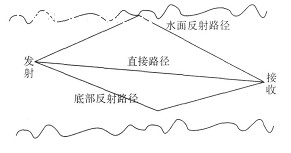
\includegraphics[width=0.5\linewidth]{figures/channel}
\begin{tikzpicture}
\draw 
	node[left] at (2,-2) {\xiaowu 发射}
	node[right] at (8,-3) {\xiaowu 接收};
\draw plot[smooth,tension=.9] coordinates {(0.000000,0.292632) (0.500000,0.274862) (1.000000,0.458597) (1.500000,0.142920) (2.000000,0.378600) (2.500000,0.376865) (3.000000,0.190223) (3.500000,0.283911) (4.000000,0.037927) (4.500000,0.026975) (5.000000,0.265399) (5.500000,0.389584) (6.000000,0.467005) (6.500000,0.064953) (7.000000,0.284412) (7.500000,0.234695) (8.000000,0.005951) (8.500000,0.168561) (9.000000,0.081091) (9.500000,0.397142) (10.000000,0.155608)};

\draw plot[smooth,tension=.9] coordinates {(0.000000,-4.735733) (0.500000,-4.917176) (1.000000,-4.699009) (1.500000,-4.868514) (2.000000,-4.672960) (2.500000,-4.655393) (3.000000,-4.625924) (3.500000,-4.774729) (4.000000,-4.958089) (4.500000,-4.885512) (5.000000,-4.543331) (5.500000,-4.923811) (6.000000,-4.587092) (6.500000,-4.730829) (7.000000,-4.501933) (7.500000,-4.960912) (8.000000,-4.778661) (8.500000,-4.946674) (9.000000,-4.519051) (9.500000,-4.997683) (10.000000,-4.612545) };

\draw[->] (2,-2) --node[below] {\xiaowu 海底反射路径} (5,-4.54) --  (8,-3);
\draw[->] (2,-2) -- node[above] {\xiaowu 直达路径} (8,-3);
\draw[->] (2,-2) -- (4.5,0.027) --node[above] {\xiaowu 海面反射路径} (8,-3);
\end{tikzpicture}
\caption{水声多途信道}
\label{fig:channel}
\end{figure}

\subsection{时变与空变}
水声信道的特性还会随着时间空间的变化而变化。造成时变特性的原因有很多,比如:收发双方的相对运动、水下鱼群的运动、水温的变化、涡流运动等。水声信道在不同水域(如港口和浅海)甚至相同水域(如深海的海面附近或者海底附近)的信道特性都不一样,其原因有:声速分布差异、噪声源种类不一等。

\subsection{多普勒效应}
当发射端和接收端之间存在相对运动时,就会出现多普勒效应,发射信号与接收信号在时域上会出现压缩或者扩展,在频域上表现为频率的平移(增大或者减小)。由于电磁波的传播速度为光速,无线电的多普勒效应要比水声信号的多普勒效应小得多。以运行时速为350km/h的高铁列车为例,其与通信基站之间的最大多普勒因子为$6.5\times10^{-7}$,而运行速度为3节(5.6km/h)的船舶与水下通信节点的最大多普勒因子为$2\times10^{-3}$。

%\subsection{传输距离、带宽和信噪比}
%传输损耗由能量扩散和声吸收引起。能量扩散仅依赖于传播距离,吸收损失不仅与传播距离有关,而且与频率有关,从而限制了传输的带宽。


\section{水声通信系统发展及现状}
\subsection{水声通信系统发展历程}
水声通信技术诞生于上世纪中叶,和其他信号
处理技术的发展趋势相同,也经历了从最初的模拟
通信阶段到现如今的数字通信阶段的过程。总的来
说,水声通信,特别是高速水声通信,近十几年的发
展趋势是由非相干通信向相干通信发展,并且随着
硬件水平、信号处理芯片计算能力的不断提高,水声
通信的调制方式、信号处理算法等都在逐渐使用各
种新的、复杂的技术,比如空间调制技术、自适应均
衡技术、盲均衡技术、分集接收技术等\citeup{catipovic1989acoustic,stojanovic1996recent,proakis1991adaptive,hinton1992adaptive}。

现在,水声通信已经发展到建立水声网络的阶
段\citeup{johnson1994design,lapierre2001design,yeo1999analysis,xie2001network}。
当前水声通信的目标是建立水下自治采样
网络(AOSN)。这种网络能够提供多个网络节点间
交换数据的功能,与此同时,也己经提出了能够传输
包括图像、数据、控制命令、语言等多种信息的水声
局域网络协议\citeup{蔡惠智2006第八讲}。

1914年英国成功研制出水声电报系统被视为水声通信的开端,第一个具有实际意义的水声通信系统是1945年美国研制的水下电话。此后,更多使用模拟单边带或着幅度调制的通信系统被开发出来。如美国通用公司研制的AN/WQC-2A水声通信机,英国研制的用于潜艇和水面舰艇的G732MK \uppercase\expandafter{\romannumeral2} 型舰艇水声通信机,法国汤姆逊·辛特尔公司研制的用于潜艇的TSMS121A和用于水面舰艇的TSMS121B水声电话,以及我国的660型声纳均是采用单边带调频方式进行水下语音通信。

\subsection{国内外水声通信系统研究现状}
水声通信多用于军事用途,西方一些国家对水声通信领域研究很是重视,包括NUMC(美国海军水下作战中心)、ONR(美国海军研究局)、NIO(英国海洋研究所)、MIT(美国麻省理工大学)、英国伯明翰大学等在内的多家研究机构和高等院校投入大量人力物力研究水声通信领域。表\ref{tab:intro:Tab1}列出了近年来国外研制的一些水声通信系统。
\begin{table}[!htbp]
	\small
	\centering 
	\TableCaption{国外研制的一些水声通信系统}
	\label{tab:intro:Tab1}
	\tabulinesep = ^1mm_1mm 
	\begin{tabu} to \textwidth{X[-3,c,m]|X[c,m]|X[-2,c,m]|X[-2,c,m]|X[c,m]|X[c,m]|X[-2,c,m]}
		\specialrule{1.5pt}{0pt}{0pt}
		公司 & 数据率 /kbps & 适用环境 & 通信方法 & 载频 & 码间干扰补偿 & 应用邻域 \\
		\hline
		Dstasoic公司 & 1.2 & 水平、垂直 & 16$\times$4-FSK & 15kHz & N/A & 水声遥控 \\
		\hline
		Micrilor公司 & 0.6 & 浅海1km & 2-DPSK          & 30kHz 100kHz & 直接序列扩频 & 水声遥控 \\
		\hline
		日本OKI电气公司 & 500 & 浅海60m & 16-QAM & 1MHz & LMS & 机器人遥控 \\
		\hline
		ENST-Br.IFREMEF & 6 & 水池 & 4-DPSK & N/A  &  判决反馈均衡 & 语音通信 \\
		\hline
		日本海洋科技学术中心 & 16 & 垂直6.5km & 4-DPSK & 20kHz & LMS & 图像通信 \\
		\hline
		WoodsHole海洋研究所 & 5 & 冰层下浅水信道 & QPSK & 15kHz & 判决反馈均衡 & 水声遥控 \\
		\hline 
		EVOLOGIC公司 & 6.5 & 水平8km 垂直200m & N/A & N/A & N/A &民用通信 \\
		\hline
		DevelLogics公司 & 7.6 & 浅海水平2.2km & MDPSK & N/A & N/A & 民用通信\\
		\specialrule{1.5pt}{0pt}{0pt}
	\end{tabu}
\end{table}

国内的水声通信领域研究起步较晚,20世纪80年代开始,包括哈尔滨工程大学、中科院声学所、厦门大学等开始研究现代的水声通信系统。直到90年代末,中船重工715研究所、西北工业大学、东南大学先后开始了水声通信的研究。表\ref{tab:intro:Tab2}列出了这些研究机构的一些研究成果。
\begin{table}[!htbp]
	\small
	\centering 
	\TableCaption{国内研制的一些水声通信系统}
	\label{tab:intro:Tab2}
	\tabulinesep = ^1mm_1mm 
	\begin{tabu} to \textwidth{X[c,m]|X[-2,c,m]|X[-2,c,m]|X[-2,c,m]|X[-3,c,m]|X[-3,c,m]}
		\specialrule{1.5pt}{0pt}{0pt}
		时间 & 完成单位 & 通信方法 & 编码方式 & 指标 & 实验场所 \\
		\hline
%		2007 &西北工业大学 & FH-MFSK和$\pi/4$-DPSK & CELP码激励线性预测编码 & 误码率小于$10^{-3}$ & 水池实验 \\
%		\hline
%		2008 & 哈尔滨工程大学 & OFDM & MB(AMBE-2000) & N/A & N/A \\
%		\hline
%		2008 & 厦门大学 & 扩频通信FSK调制 & N/A & 3km,200bit/s,误码率约$10^{-3}$ & 厦门港 \\
%		\hline
%		2008 & 哈尔滨工程大学 & QPSK & MELP & 6.4kbps & 水池实验 \\
%		\hline
%		2008 & 中国科学院声学研究所 & BPSK或QPSK & MELP &6km处误码0.4\%~11km处误码2.1\% & 黄海海试 \\
%		\hline
%		2009 & 北京理工大学 & MFSK & N/A & 通信距离大于2km误码小于$10^{-3}$ & 水池长2km深1.5m \\
%		\hline
		2010 & 海军指挥学院和东南大学 & 4-DPSK & CELP &N/A &水池实验 \\
		\hline
		2011 & 哈尔滨工程大学 & IFFT/FFT & MBE(AMBE-2000) & N/A &N/A \\
		\hline
		2012 & 海军工程大学、哈尔滨工程大学 & OFDM & MBE(AMBE-2000) & 4.6kbps & 哈尔滨工程大学消声水池 \\
		\hline
		2012 & 中国科学院声学研究所 & 单边带调制 & N/A & N/A & 7km深度潜器和母船通信 \\
		\hline
		2013 & 厦门大学 & OFDM & MELP & 2.4kbps & 水池实验 \\
		\hline
		2013 & 哈尔滨工程大学 & OFDM & N/A & 2.4kbps,2km & 湖试 \\
		\hline
		2013 & 中国科学院大学 & QPSK & MELP & 10km,误码率$2.5\times10^{-4}$ & 黄海海试\\
		\hline
		2014 & 哈尔滨工程大学 & CSS-OFDM-VTRM & PSK & 1km误码率0.0108 & 湖试 \\
		\hline
		2015 & 厦门大学 & 扩频通信 & DS-DBPSK & N/A & 湖试 \\
		\specialrule{1.5pt}{0pt}{0pt}
	\end{tabu}
\end{table}

\section{水声扩频通信系统研究现状}
%相比于传统的水声通信方式,扩频通信有诸多有点。首先,扩频通信的码元类似噪声的特性使其在没有先验知识的情况下很难被检测到。其次,扩频带来的扩频增益使淹没在噪声中的信号也能狗被检测到,远距离、低信噪比时扩频通信表现更出色。最后,扩频通信系统可以用不同的扩频序列来区分不同用户使其能够支持多用户接入的能力,以此增大了信道的软容量。
%
%除了传统的直接序列扩频(DSSS)外,近些年还逐渐发展起了M元扩频和多通道扩频等不同形式的通信系统。文献\cite{王海斌2004混沌调频}提出了一种混沌调频M元远程水声通信技术,其通信距离为3km,通信速率为6.3bps,误码率为$8.0\times10^{-4}$。Paul Hursky等人在2006年研究了基于M元的点对点水声通信技术,其通信距离能达到1.2km-5.4km\citeup{hursky2006point}。
和传统的水声通信方式相比,扩频通信有着许多的优点,使其在军用民用领域获得了广泛的应用。首先,类似于噪声的特性使其在没有先验知识的情况下很难被检测到,扩频增益使其可以在很低的信噪比下工作并获得了很低的截获概率。其次,扩频信号的低功率密度谱特性使其能够有效的减少有意和无意的单频和宽带信号的干扰。这种抗干扰的能力也使其容许在码域上进行复用,不以带宽为代价获得通信速率的提高,这对水声通信这种严重带限的系统显然是有意义的。最后,扩频系统有着多址接入的能力,每个用户使用其自己独有的扩频序列来进行区分地址,其软容量使其在不同的信道条件和信噪比下可以获得不同的用户数支持度。
\subsection{M元扩频研究现状}
M元扩频和传统的DSSS扩频相比,有效的减少了扩频增益对通信速率的制约,极大的提高了每符号携带的通信速率。这种方式可以提高系统抗噪声能力,也就是可以提高系统的通信距离。同时,对于没有进行相位调制的M元扩频,可以用非相干和相干两种接收机结构对其进行处理,和DSSS相比,增加了接收机的灵活性\citeup{周锋2012水声扩频通信关键技术研究}。

文献\cite{王海斌2004混沌调频}提出了一种基于混沌调频M元方式的远程水声通信技术。在南海进行了可行性实验,通信距离为31km,使用混沌序列的长度为127,带宽为50Hz,发射声源级186dB,其通信速率为6.3bps,得到的误码率为 。

2006年,文献\cite{hursky2006point}研究了使用扩频通信方式的点对点水声通信技术,其中,信息调制使用的是PPM和差分相移键控(DPSK),信号的形式使用的是Gold序列,并与被动相位合并技术相结合。实验使用的带宽为8k-16kHz,其通信距离为1.2k-5.4km。

2009年,西北工业大学的何成兵,黄建国和韩晶等提出了循环移位扩频水声通信技术\citeup{何成兵2009循环移位扩频水声通信},针对扩频序列优良的循环自相关特性,把信息调制到码元相位上,在发射端,进行循环移位编码,在中远程湖上实验中,15km的距离上,实现了438bps通信速率的传输,误码率为$10^{-2}$到$10^{-3}$。

2010年,文献\cite{zhang2010efficient}提出了一种正交载波调制的PPM方案来传输信息,一条作为参考序列,令一条作为参考序列的移位,这可以看做是一种差分的M元PPM 方案。实验参数为9.6kHz的中心频率,3kHz的带宽。在0.243k-0.776km的距离下,在主动相位合并接收机(PPCR)的框架下实现了最差0.17\%误符号率的通信。

2012年,文献\cite{zhang2012experimental}进行了远距离水声通信的实验研究,在远距离水声通信的情况下,接收的水声信号有着较低的SNR,文章采用两个最大长度序列(也就是m序列)在时域上相叠加的方式,信号调制方式为码元循环移位键控。使用三种接收机的结构来展现其结果,一种是相关接收,一种是被动相位合并(PPC)接收机,还有一种是时间反转接收机,并比较了三种接收在10km距离上的实验结果。实验使用的频带为11k-13kHz,采样率为96kHz,发射声源级为187dB,可以得到最优情况的误码率为 。
\subsection{多通道扩频研究现状}
多通道扩频通信技术可以看做是一种同步的CDMA系统,它是建立在点对点通信的基础之上。M元扩频对通信速率的提高是有限度的,而多通道对通信速率的提高随着通道数的增加而成倍增加。在CDMA系统中,一些高级的信道估计算法被研究,它们有基于Kalman的估计器[A\citeup{iltis1994ekf,iltis1990joint,iltis1991digital}和严重信道衰落情况下的基于信号子空间的方法\citeup{amleh2003algebraic,affes2002interference}。

2006年,文献\cite{韩晶2006正交}中研究了正交M元/DS扩频水声通信技术,使用M元和DS相结合的通信方式,其接收机的部分,M元部分采用非相干技术,DS部分采用差分技术。在25km的通信距离上,4kHz带宽和0dB左右的接收信噪比下,采用Rake接收技术,在63和127长度的Gold序列下实现了480符号信息量的无误码传输,通信速率为220.5bps和381.0bps。

2007年,殷敬伟,惠俊英和王逸林等提出的M元混沌扩频多通道Pattern时延差编码水声通信技术\citeup{殷敬伟2007m},该系统使用优选的混沌序列,使用多通道的方式提高通信速率,在6k-9kHz的带宽内,600-3490m的距离上,在3-8通道,实现了150-400bps通信速率上0-4.1\%BER的有效传输。

文献\cite{惠俊英2008分组}研究了分组M元扩频Pattern 时延差编码水声通信技术,分组M元在一定程度上可以看做是多通道M元技术。它采用扩频码进行并行传输的方法有效的提高了Pattern时延差编码水声通信的通信速率。文献\cite{jing2006underwater}仿真研究了在4路并行Pattern时延差编码水声通信技术在8kHz带宽下的研究结果,其可以达到1kbps的通信速率,这也为高速率扩频水声通信技术提供了一些解决的思路。

2009年,文献\cite{yang2009interference}对CDMA水声通信中的干扰抑制技术进行了研究。文章针对多用户通信中的远近效应,一种坐标归零的多维空间删除方法被使用。通过利用基于干扰序列的快速Walsh-Hadamard变换,干扰信号可以被降低,并被坐标归零消除,再对剩余的部分进行一个反变换。并用这种方法与传统的方法进行了比较。

2012年,哈尔滨工程大学的殷敬伟,杨森和杜鹏宇等提出的基于单矢量有源平均声强器的码分多址水声通信\citeup{殷敬伟2011基于单矢量有源平均声强器的码分多址水声通},将矢量传感技术和扩频技术有效的结合在一起。在湖试实验中,5k-7kHz的带宽,在400-2000m的距离下,实现了3用户水声通信,并达到了$10^{-2}$量级的误码率。

\section{本文主要研究内容}
本文旨在基于低功耗单片机MSP432上实现扩频通信算法。根据MSP432的特性,对算法的各个阶段进行优化。MSP43时德州仪器(TI)公司刚推出市场的一款兼具低功耗和高性能(相比于MSP430)的基于ARM Cortex M4F内核的单片机。MSP432的M4F内核具有一个浮点运算单元,以及支持最高48MHz的主频。MSP432的功耗低至90uA/MHz,并且具有4个等级低功耗模式。

ARM Cortex M4F内核支持ARM CMSIS-DSP程序库,库中包含了用于数字信号处理的常用算法的快速实现,例如:FFT、FIR、正余弦函数、复数运算等。利用CMSIS-DSP库设计扩频算法将大大降低程序编写难度,而且能保证耗时运算(如FFT)的高效率。

本文还是实现了二阶差分检测算法,将其应用与扩频通信系统中。二阶差分检测能够抵抗一定程度的多普勒,简化接收机结构。但同时二阶差分检测也有应用的局限性,例如多普勒不能太大,扩频序列长度不能太长等。

